
We put together a number of storyboards to best draw initial designs of the application. They were also used in a meeting with the library staff to exhibit our perspective on what the application will look and feel like. The below figure shows what would replace the current Contact Us page with which streamlines the user flow and routes users automatically with general questions rather than prompting a chatroom with a librarian for such questions.

\begin{figure}[H]
    \centering
    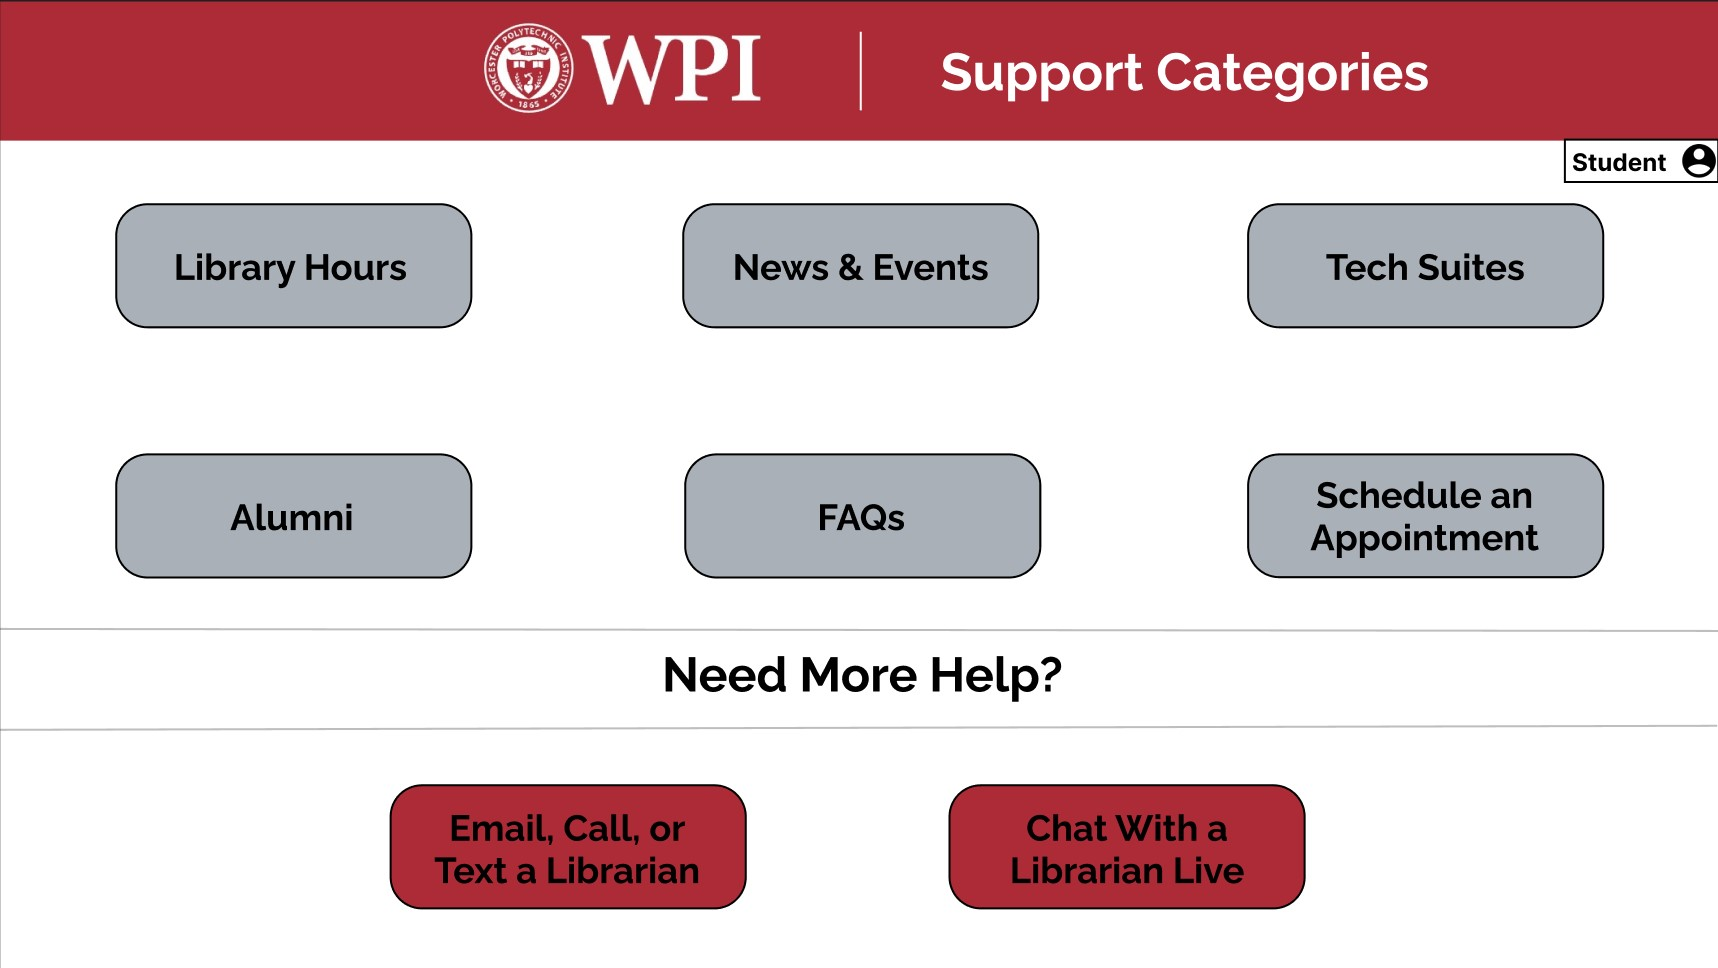
\includegraphics[width=0.5\textwidth]{chapters/methodology/conceptual_designs/MQP Main Page}
    \caption{Student view of the Contact Us page.}
\end{figure}

The figure below showcases a rudimentary iteration of what the chatroom interface is expected to look like. Here, from the librarian's perspective, the user is supplied with a number of convenient features ranging from automated prompt responses, chat duration, file uploading, and more.

\begin{figure}[H]
    \centering
    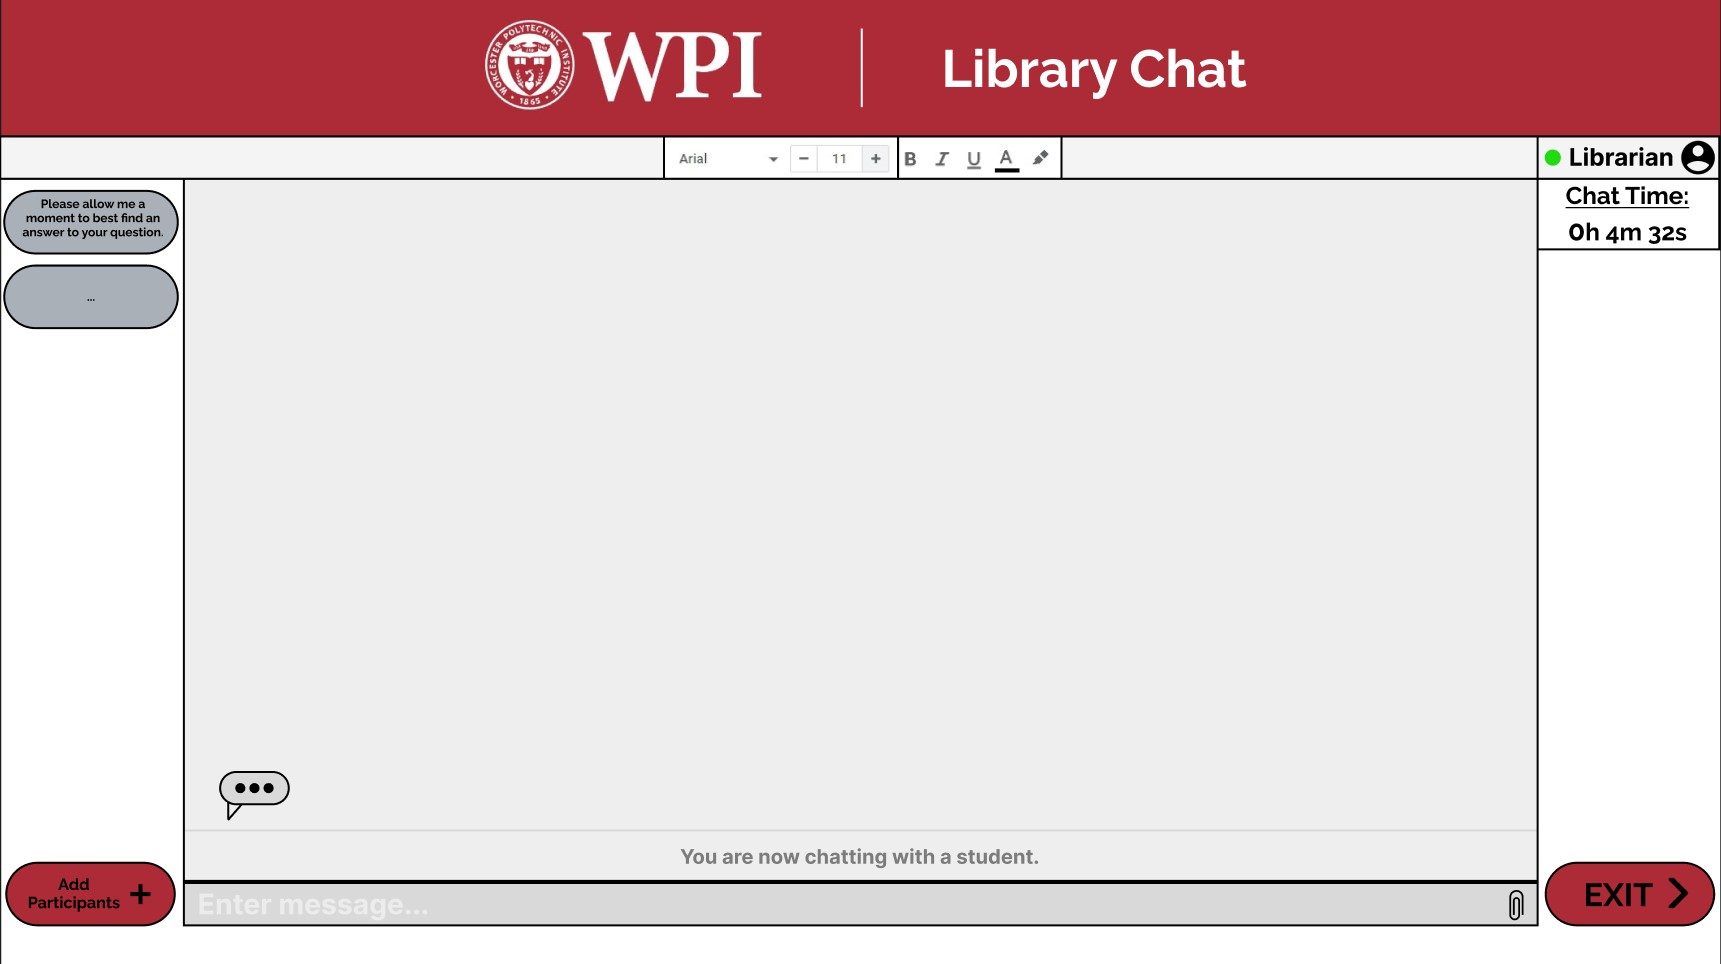
\includegraphics[width=0.5\textwidth]{chapters/methodology/conceptual_designs/MQP Librarian Chat.jpg}
    \caption{Librarian view of a chatroom.}
\end{figure}
